\newcommand{\chapter}[2][]{
	\newcommand{\chapname}{#2}
	\begin{flushleft}
		\begin{minipage}[t]{\linewidth}
			
\includegraphics[height=1cm]{hdht-logo.png}
			\hspace{0pt}	
			\sffamily\bfseries\large Bài  20.
			\begin{flushleft}
				\LARGE\bfseries #1
			\end{flushleft}
		\end{minipage}
	\end{flushleft}
	\vspace{1cm}
	\normalfont\normalsize
}
\chapter[Phương pháp phân tích lực \\giải bài toán động lực học]{Phương pháp phân tích lực giải bài toán động lực học}
\section{Phương pháp chung}

Phương pháp phân tích lực giải bài toán động lực học là phương pháp khảo sát chuyển động của các vật dựa trên cơ sở các định luật Newton. Phương pháp phân tích lực bao gồm các bước cơ bản sau:
	 \begin{enumerate}[label=\textbf{\arabic*}.]
	 	\item \textbf{Xác định các lực tác dụng lên vật hoặc hệ vật và vẽ giản đồ lực.}
	 		
	 		Các lực cần được xác định rõ điểm đặt, phương, chiều, độ lớn. Các lực thường gặp là: 
	 			\begin{itemize}
	 				\item Các lực do các trường lực gây ra như trường hấp dẫn, điện trường, từ trường, $\ldots$
	 				\item Các lực do liên kết giữa các vật trong hệ: lực căng dây, lực đàn hồi, $\ldots$
	 				\item Các lực do tiếp xúc giữa vật và các vật khác: áp lực, phản lực, lực ma sát.
	 			\end{itemize}
	 	\item \textbf{Viết phương trình định luật II Newton cho vật hoặc hệ vật }
	 	
	 		Phương trình viết ở dạng vectơ 
	 			\begin{align}
	 				\sum\vec{F}=m\vec{a},
	 			\end{align}
 			trong đó $\sum\vec{F}$ là tổng vectơ các lực tác dụng lên vật hoặc hệ vật, $m$ là khối lượng của vật hoặc hệ vật tương ứng. 
 			
 			Trong trường hợp hệ gồm nhiều vật, ứng với mỗi vật có thể viết một phương trình định luật II Newton tương ứng
 				$$\begin{cases}
 					m_1 \vec{a}_1 = \Sigma \vec{F}_1\\
 					m_2 \vec{a}_2 = \Sigma \vec{F}_2\\
 					\ldots\\
 					m_n \vec{a}_n = \Sigma \vec{F}_n\\
 				\end{cases}$$
 			trong đó  $\Sigma \vec{F}_n$ là tổng các lực tác dụng vào vật thứ $n$, $m_n$ là khối lượng của vật thứ $n$ tương ứng. 
 			 
	 	\item \textbf{Giải phương trình định luật II Newton }
	 		
	 		Phương trình định luật II Newton là phương trình vectơ. Một trong những cách phổ biến để giải phương trình này là chiếu phương trình này lên các trục tọa độ và giải hệ các phương trình hình chiếu. 
	 		
	 		Đối với các bài hệ vật, ta có thể chọn một hệ trục chung cho cả hệ, hoặc ứng với mỗi vật lại chọn một hệ trục riêng. Khi đó mỗi phương trình định luật II Newton ứng với mỗi vật cần phải được chiếu lên hệ trục tương ứng. Ngoài ra ta cũng cần xác định rõ mối liên hệ gia tốc giữa các vật trong hệ, thường được xác định qua liên hệ tọa độ các vật. 
	\end{enumerate}

	\manatip{Phản lực $\vec{N}$ luôn vuông góc với mặt tiếp xúc, còn lực ma sát luôn có phương tiếp tuyến mặt tiếp xúc, nên ta thường chọn hệ trục O$xy$ có trục O$y$ vuông góc mặt tiếp xúc, O$x$ song song mặt tiếp xúc. Như vậy, phương trình hình chiếu định luật II Newton trên trục O$y$ cho phép ta xác định được biểu thức của phản lực $N$. Thay biểu thức này vào lực ma sát $F_\text{ms}=\mu N$ trong phương trình hình chiếu trên trục O$x$ sẽ giúp ta giải được bài toán.}

\section{Minh họa phương pháp phân tích lực trong việc giải bài toán hệ một vật}
	\viduii{3}{
		Một vật nhỏ khối lượng $m$ chuyển động theo trục O$x$ trên mặt phẳng nằm ngang dưới tác dụng của lực kéo $\vec F$ chếch lên theo hướng hợp với O$x$ một góc $\alpha>0$. Hệ số ma sát trượt trên mặt ngang bằng $\mu_\text{t}$. Xác định gia tốc chuyển động của vật
}
{	\begin{center}
		\textbf{Hướng dẫn giải}
	\end{center}
	\begin{center}
		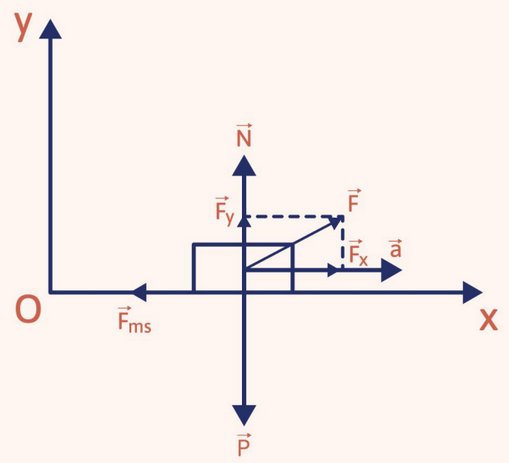
\includegraphics[scale=0.5]{../figs/G10-17-1}
	\end{center}
	
	\begin{itemize}
		\item Các lực tác dụng lên vật gồm lực kéo $\vec F$, lực ma sát $\vec F_\text{ms}$, trong lực $\vec P$, phản lực $\vec N$ được thể hiện trên giản đồ. 
		
		\item Phương trình định luật II Newton có dạng 
		\begin{equation}\label{*}
			\vec F +\vec F_\text{ms} + \vec P + \vec N = m \vec a
		\end{equation}
		
		\item Chọn hệ trục tọa độ: O$x$ nằm ngang, O$y$ thẳng đứng hướng lên trên và chiếu phương trình \eqref{*} lên các trục tọa độ đã chọn:
			\begin{itemize}
				\item Chiếu (\ref{*}) lên O$y$:
				\begin{equation}\label{***}
					F_y + N - P = 0 \\
					\quad\Rightarrow\quad N = P - \sin \alpha
				\end{equation}
				\item Chiếu ($\ref{*}$) lên O$x$:
					\begin{equation}\label{**}
						F_x - F_\text{ms} = ma \\
						\quad\Rightarrow\quad F \cos \alpha - \mu_\text{t} N = ma
					\end{equation}
			\end{itemize}
		Thay $N = P - \sin \alpha$ từ phương trình \eqref{***} vào phương trình \eqref{**}, ta tính được 
			$$a=\dfrac{F \cos \alpha - \mu_\text{t} (P-\sin \alpha)}{m}.$$
	\end{itemize}
}
	\viduii{3}{
	Một chiếc hộp gỗ được thả trượt không vận tốc ban đầu, từ đầu trên của một tấm gỗ dài $L=\SI{2}{m}$. Tấm gỗ đặt nghiêng $30^\circ$ so với phương ngang. Hệ số ma sát giữa đáy hộp và mặt gỗ là $\SI{0.2}{}$. Lấy $g=\SI{9.8}{m/s^2}$. Hỏi sau bao lâu thì hộp trượt xuống đến đầu dưới của tấm gỗ?
}
{	\begin{center}
		\textbf{Hướng dẫn giải}
	\end{center}
	
	\begin{center}
		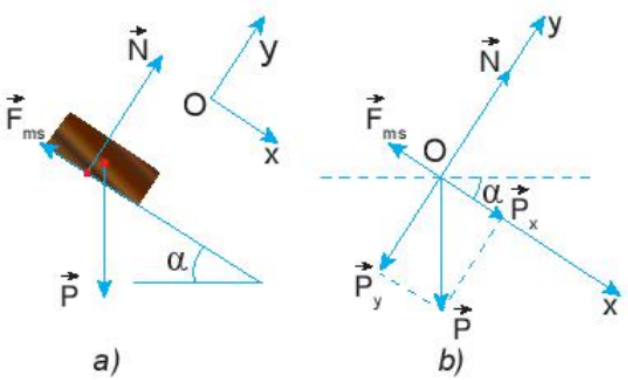
\includegraphics[scale=0.5]{../figs/G10-17-3}
	\end{center}
	
	\begin{itemize}
		\item Hộp gỗ (coi là chất điểm) chịu tác dụng của ba lực: trọng lực $\vec P$, phản lực $\vec N$ và lực ma sát $\vec F_\text{ms}$ như ở hình bên trái.
		
		\item Phương trình định luật II Niu-tơn:
		\begin{equation}\label{10}
			\vec F_\text{ms} + \vec P_x + \vec P_y + \vec N = m \vec a
		\end{equation}
	
		\item Chọn hệ trục tọa độ: O$x$, O$y$ như hình vẽ. Phân tích trọng lực $\vec P$ thành hai lực thành phần $\vec P_x$, $\vec P_y$ như trong hình bên phải.
		
		Chiếu các vectơ lực lên các trục tọa độ đã chọn:
			\begin{itemize}
				\item Chiếu (\ref{10}) lên O$y$:
					\begin{equation}\label{12}
						N - mg \cos \alpha = 0 \quad\Rightarrow N = mg\cos\alpha \quad\Rightarrow F_\text{ms}=\mu N=\mu mg \cos\alpha.
					\end{equation}
				\item Chiếu ($\ref{10}$) lên O$x$:
					\begin{equation}\label{11}
						mg \sin \alpha - F_\text{ms} = ma \quad\Rightarrow a= g(\sin \alpha - \mu \cos \alpha)
					\end{equation}
			\end{itemize}

		Thay số, ta được $a \approx \SI{3.2}{\meter/\second}$. Vậy hộp trượt xuống với gia tốc $a=\SI{3.2}{\meter/\second^2}$, cùng chiều với trục O$x$.
		
		\item Áp dụng công thức xác định thời gian trong chuyển động thẳng biến đổi đều:
		$$L=\dfrac{1}{2}at^2\quad\Rightarrow\quad t=\sqrt{\dfrac{2L}{a}} \approx \SI{1.1}{\second}$$
	\end{itemize}
}
\section{Minh họa phương pháp động lực học trong việc giải bài toán hệ nhiều vật}
	\viduii{4}{Hai vật 1 và 2 có thể trượt trên mặt bàn nằm ngang và được nối với nhau bằng dây không dãn, khối lượng dây không đáng kể. Khối lượng của các vật là $m_1 = \SI{2}{kg}$, $m_2=\SI{1}{kg}$. Tác dụng vào vật 1 lực $F=\SI{9}{N}$ theo phương song song với mặt bàn. Hệ số ma sát giữa hai vật với mặt bàn là $\mu=\SI{0.2}{}$. Lấy $g=\SI{10}{m/s^2}$. Hãy tính gia tốc chuyển động của các vật.
}
{	\begin{center}
		\textbf{Hướng dẫn giải}
	\end{center}
	
	\begin{center}
		\begin{tikzpicture}
			\node[anchor=south west,inner sep=0] at (0,0) {\includegraphics[scale=0.7]{G10-17-2}};
			\draw[red,thick,-stealth] (6.8,1.35) -- (5.9,1.35);
			\node[below] at (5.9,1.35) {$\vec{\text{F}}_{\text{ms}_1}$};
		\end{tikzpicture}
%	\includegraphics[scale=0.5]{../figs/G10-17-2}
	\end{center}

	\begin{itemize}
		\item Đối với vật 1:
		\begin{equation}\label{1}
			\vec P_1 + \vec N_1 + \vec T_1 + \vec F_\text{ms1} + \vec F = m_1 \vec a_1
		\end{equation}
	
		Chiếu (\ref{1}) xuống O$x$: $F - T_1 - F_\text{ms1} = m_1 a_1$.
		
		Chiếu (\ref{1}) xuống O$y$: $-m_1 g + N_1 = 0$.
		
		Với $F_\text{ms1} = \mu N_1 = \mu m_1 g$, suy ra:
		\begin{equation}\label{2}
			F-T_1 - \mu m_1 g = m_1 a_1
		\end{equation}
		\item Đối với vật 2:
				\begin{equation}\label{3}
			\vec P_2 + \vec N_2 + \vec T_2 + \vec F_\text{ms2} + \vec F = m_2 \vec a_2
		\end{equation}
		
		Chiếu (\ref{3}) xuống O$x$: $T_2 - F_\text{ms2} = m_2 a_2$.
		
		Chiếu (\ref{3}) xuống O$y$: $-m_2 g + N_2 = 0$.
		
		Với $F_\text{ms2} = \mu N_2 = \mu m_2 g$, suy ra:
		\begin{equation}\label{4}
			T_2 - \mu m_2 g = m_2 a_2
		\end{equation}
	
		\item Do khối lượng dây không đáng kể nên $T_1 = T_2 = T$, do dây không dãn nên $a_1 = a_2 = a$.
		
		Biến đổi (\ref{2}), ta được:
		\begin{equation}\label{5}
			F - T - \mu m_1 g = m_1 a
		\end{equation}
	
		Biến đổi (\ref{4}), ta được:
		\begin{equation}\label{6}
			T - \mu m_2 g= m_2 a
		\end{equation}
	
		\item Cộng (\ref{5}) và (\ref{6}), ta được:
		\begin{equation*}
			F - \mu (m_1 + m_2) g = (m_1 + m_2) a \\
			\Rightarrow a = \dfrac{F - \mu (m_1 + m_2)g}{m_1 + m_2} = \SI{1}{m/s^2}
		\end{equation*}
	\end{itemize}
}